% Chapter Template

\chapter{Design and Development} % Main chapter title

\label{DesignAndDevelopment} % Change X to a consecutive number; for referencing this chapter elsewhere, use \ref{ChapterX}

\lhead{Chapter \ref{DesignAndDevelopment}. \emph{Design and Development}} % Change X to a consecutive number; this is for the header on each page - perhaps a shortened title

%----------------------------------------------------------------------------------------
%	SECTION 1
%----------------------------------------------------------------------------------------

\section{The design of \theartefact}
%%%%%%%%%%%%%%%%%%%%%%%%%%%%%%%%%%%%%%%%%%%%%%%%%%%%%%%%%%%%%%%%%%%%%%%%%%%%%%%%%%%%%%%%%
%%%%%%%%%%%%%%%%%%%%%%%%%%%%%%%%%%%%%%% TODO %%%%%%%%%%%%%%%%%%%%%%%%%%%%%%%%%%%%%%%%%%%%
%%%%%%%%%%						Intro to section							%%%%%%%%%%%%%
%%%%%%%%%%%%%%%%%%%%%%%%%%%%%%%%%%%%%%%%%%%%%%%%%%%%%%%%%%%%%%%%%%%%%%%%%%%%%%%%%%%%%%%%%

\subsection{Design}
The artefact was divided into several modules which function independently of each other.
The modules were loosely coupled so that each module could be changed or modified without affecting the other modules.
The modules that were created were:
\begin{itemize}
	\item The web front end
	\item A module that fetched and processed the HTML from the sites that the user wanted to mark up
	\item A module for fetching possible disambiguating terms from lexitags
	\item A module for finding the best fit mappings for SUMO and schema.org
	\item A module for finding the best fit mappings from DBPedia to schema.org
	\item A module that puts the document back in its initial state and saves it to a persisten storage
\end{itemize}

\section{Run through of common use}
Common use case:
User comes to site -> Basic site generated from template on server

The user enters URL of page to tag:
\begin{itemize}
	\item URL gets sent to proxy module on server
	\item Proxy fetches the HTML of the target URL
	\item Proxy comments out script and iframe tags
	\item Proxy replaces relative image URIs with absolute image URIs.
	\item Proxy sends back an object containing the sites head and body tag
	\item The content of the body tag is used to populate the content container in the web app.
\end{itemize}
The user highlights a word on the page to add metadata to:
\begin{itemize}
	\item The text of the highlighted selection gets sent to the lexitags server for disambiguation
	\item The results from lexitags are filtered
	\begin{itemize}
		\item If the results contain WordNet terms, then the DBPedia results are filtered away
	\end{itemize}
	\item The results are then sorted
	\begin{itemize}
		\item Primarily by source, WordNet terms first, then the first and second level schema.org terms
		\item Secondarily they are sorted lexically
	\end{itemize}
	\item Then the results are displayed on the web page. If the user cannot find a match with the highlighted text,
	it is posible to write your own word into a search box.
	The semantics of this word will then be linked to the highlighted text.
\end{itemize}
The user click the sense of the word which match the intended semantics of the highlighted word
\begin{itemize}
	\item The term, either a WN synset or a DBP entity gets sent to the mapping module on the server
	\item The mapping module find the mappings into other ontologies
		that most closely matches the semantics of the term.
	\item The server returns the entity types that best fit the term, and their namespaces
		\item If no schema.org mapping is found, schema:Thing is returned as it is always correct.
	\item The web app adds a tag which surrounds the selected text, and adds the entity value to it using RDFa
		\item This new tag contains keywords which will highlight it on the page
	\item The web app then asks the server for the schema.org properties of it's schema type(s).
	\item The server returns all the applicable properties
	\item The web app adds all the returned properties to the markup of the page with empty values
\end{itemize}
The user clicks a marked up section
\begin{itemize}
	\item The web app displays all the possible attributes the section can have
	\begin{itemize}
		\item If values have already been inserted, these are shown as the default values
	\end{itemize}
	\item The user inputs the values the attributes should have
	\item When the submit button is click, the attributes get updated to the correct values
\end{itemize}
The user clicks the export button
\begin{itemize}
	\item The html on the page is cleaned
	\begin{itemize}
		\item Temporary markup(tooltips, popover) is removed
		\item Attributes without values are removed
	\end{itemize}
	\item The html is sent to the server
	\begin{itemize}
		\item The exporter comments in the script and iframe tags
		\item The html is put in the database
	\end{itemize}
	\item The server returns the id of the new web page
	\item The web app displays the URL to the new marked up website.
\end{itemize}
\subsection{Designing the algorithms}
We will now describe the two algorithms that were developed to find mappings between the WordNet synsets and the ontologies.
We use two axes for navigating the WordNet graph, the hypernymes and the hyponymes.
As described in \ref{TheoryWordNet}, a hypernyme can be described as category words into which more specialized words fall.
Hyponyme is the inverse relation, where a hyponyme is a word which can be generalized into some more general category.
For simplicity we will also use one additional term.
We will use \emph{sibling} to refere to words which are hyponymes of a words hypernyme.
An example( see figure \ref{Hyponyme}, page \pageref{Hyponyme})
would be that \{dog\} has the hypernyme \{domestic\_animal\}, which again have the hyponyme \{cat\},
\{cat\} would then be considered a sibling term of \{dog\}.


Our hopes for this mapping tree is that in the cases where there is no direct mapping from the synset to a term in the
ontologies we are mapping to, we can always preserve the semantics of the synset by using one of the synsets ancestors.
For the siblings we hope that if we find a mapping,
then the parent term of the term we have mapped to in the ontology will correspond to the meaning of the synset.
Both these propositions will be tested as a part of the work with the thesis.

The algorithms define different orders of looking at the synsets

\subsubsection{Generating the search tree}
The first step of the algorithm is the same for both algorithms.
A search tree is generated using a perl script
\footnote{Perl script found at \url{https://raw.github.com/EivindEE/SemTag/master/scripts/parents.pl}.}.

\begin{figure}[h]
    \begin{center}
        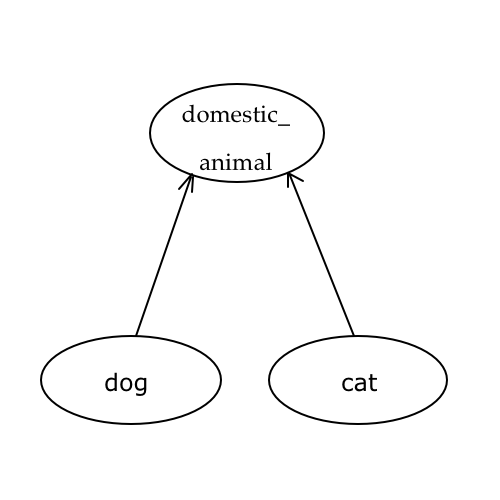
\includegraphics[width=0.60\textwidth]{Hyponyme_own.png}
        \caption{The hyponyme relation, modified from \protect \citet{Miller1990}}
        \label{Hyponyme}
    \end{center}
\end{figure}



\subsubsection{The sibling first algorithm}
The sibling first algorithm traverses the search tree by first looking if there is a direct mapping from the base synset to the ontologies.
If a direct mapping is not found, it will look at the hypernyms and see if it has a mapping.
After looking at the hypernyms it will look at the sibling senses.
It will then go on to look at the hypernyms of the hypernyms, and then their sibling states.
It will continue to follow the hypernym chain upwards until there are no more hypernyms, or a mappings has been found.

\subsubsection{The ancestors first algorithm}
The ancestor first algorithm will follow the hypernym chain upwards looking for mappings.
The algorithm is written to follow the hypernym chain again, looking at the sibling senses, if no mapping is found.
But since every WordNet noun is a hyponyme of {entity}, which should map to the most general object in an ontology,
it will likely never be touched.


%----------------------------------------------------------------------------------------
%	SECTION 2
%----------------------------------------------------------------------------------------

\section{The development process}


\section{Iteration 1}
The first iteration started with getting to know the technologies, and setting up a framework
Quite some time was spent getting comfortable working with the \nom{DOM}
{The Document Object model, convention for interacting with HTML elements},
and the peculiarities of the different mainstream browsers.
At this point we also set up the server that the web app would run on.

\section{Server setup}
Setting up a basic server in node.js can be done in a single line of code,
but requires a lot of low level handeling of requests and responses
including parsing request url to find the correct handler.
We decided to instead go for express\footnote{\url{http://expressjs.com}},
a web app framework which simplifies routing requests to the correct handler and handeling static files.
%Additional benefits of using the framework included simplified logging of requests, and
It was also decided to use the jade\footnote{\url{http://jade-lang.com}}
templating language to generate the \nom{HTML}{HyperText Markup Language} that was used on the website.
Using a templating language made the distinction between structure and content clearer,
and enabled reuse of structure and content between different versions of the website during development.


\section{Representing other websites}
One of the issues that come up early was how to display the websites that the user wanted to add metadata to.
Early attempts tried using the iframe\footnote{http://www.w3.org/TR/html5/embedded-content-0.html\#the-iframe-element}
element of \nom{HTML}{HyperText Markup Language}.
Embedding the target website in an iframe was the first try as it would allow the page to display in the same maner
as it does when accessed directly.
Using the iframe element in this maner would however constitute cross-domain communication and is not allowed.

This problem was not solved in the first iteration.
After trying to find a workaround it was decided that displaying html from other websites was not essential to the work,
and that the focus should be shifted to adding markup.
The solution we landed on was to insert some placeholder text which was used for testing purposes.
This placeholder text is still displayed on the website to give visitors something to try the tool on before using it
to add markup to their own pages.

\section{Interaction method}
\label{Interaction}
When we first faced to problem of how to let users interact with the web app we felt that using the highlighting or
selection of text to be the most intuitive approach.
We also believed that this would be the simplest interaction method to implement.
The simple case of taking selected text and displaying it in the console can be implemented as in listing \ref{DOMSelection}.

\begin{lstlisting}[caption={Logging selected text}, label=DOMSelection]
	var logSelection = function () {
		console.log(window.getSelection().getRangeAt(0).toString());
	};
	document.addEventListener('mouseup', logSelection);
\end{lstlisting}

The "mouseup" event is triggered every time the user has pressed and then released the mouse pointer on the website.
This event is not available on mobile and tablet type browsers,
but adding listeners for corresponding events should not be difficult if we later see the need for this.

In the web app the selected text is sent to the web server to find possible disambiguations for the text.
The lexitags service that we use for disambiguation now is targeted towards disambiguating single words.
It does handle some composite terms and some proper nouns, but this is outside the normal use case.
The service can also become unstable when the query reaches a certain length, about 500 characters.
To circumvent this problem we do a simple check for the length of the text string.
If the length of the string is more than the longest allowed length,
the query is instead replaced with a shorter query indicating that the selection is of a larger section of text.

The response from the server is a JSON string containing the terms that were found to be possible senses of the selected text.
Each of these senses have an explanation property which gives a short textual description of the meaning of the sense.
These senses are displayed as a list on the web site.
The senses that are returned come from different sources.
They can come either from WordNet and take the form of WordNet synsets, or they can be resources from DBPedia.
Both of these can be used to generate mappings,
but the most interesting mapping for this thesis lies in generating mappings from WordNet so the synsets are given preference in the list.
Lexitags also returns the top level resources from schema.org as shown in figure \ref{TopLevelSchemaOrg}(page \pageref{TopLevelSchemaOrg}).
These are sorted to the bottom of the list as these are fallbacks for when none of the of the terms suggested for
the word turn out to be reasonable suggestions for the selected text.

To select one of the terms from the list as the meaning of the selected text the user clicks the sense in the list.
When a sense is clicked it is sent to the server to be mapped.
The servers uses the best fit algorithm described in \ref{BestFitMapping}(page \pageref{BestFitMapping}) to find the ontology references
that fits the sens best and attaches these references to the selection using RDFa.
The algorithm used to attach the metadata to the selection can handle an arbitrary amount of namespaces and references.
If there is duplication of references these will be dropped.

One of the difficult aspects of adding the metadata to the selections was making sure that the HTML was well-formed
after the metadata was inserted.
One of the rules regarding the well-formednes of a HTML document says that two elements can't overlap as in listing \ref{OverlappingHTML}.

\begin{lstlisting}[language=HTML, caption=Example of overlapping elements, label=OverlappingHTML]
	<a>
		<b>
	</a>
		</b>
\end{lstlisting}

The interaction method consists of letting the user make arbitrary selections and then adding metadata to the selection.
This could easily lead to overlapping elements in the HTML.
To avoid this malformed HTML we check the range of the selected text and see if surrounding it with a tag
containing metadata would result in a well-formed document, and modify the range if needed.
If the start and end of the selection are in the same element then adding metadata is safe.
If that is not the case we find the smallest change we need to make to the scope of the range to make it safe.
There are two general cases her, when either the start or the end of the range is in a descendant element of the other,
and when both start and end are descendants of a common element but not of each other.

In the first case we need to find out which element is the descendant of which.
We do that by following the ancestor links of each element.
When we find that either the start or end element has the other as an ancestor we use the ancestor which is the direct
child of the other element and place the start or end tag right before or after that tag, depending on which element
descended from which.

When the elements are not descendants of each other we know that they must be descendants of some other element.
If nothing else they must both be descendants of the root element.
We use a similar approach for this case as we do for the fist,
but instead of finding the ancestor which is the direct child of the other node we find the one which is a child of the
closest common node.
We then surround these elements with the metadata tag.
This metadata element is styled with a distinct color to let the user know that the text is tagged.

When the metadata element is created,
the schema.org type is sent back to the server to get a list of the possible properties of that type.
On the server we use a JSON representation of the schema.org ontology to find the properties that a type can have.
The representation we use was retrieved from \url{http://schema.rdfs.org} which is a support site that tries to
promote linked data.
For each of the types in schema.org the JSON file provides the properties specific to that type,
and all the properties it has inherited from its super types.
We combine the information about which properties a type can have with a short description of what the property represents,
and information about the range of the property, that is the range of values that are valid values of the property.
The resulting JSON object is then returned to the website.
These properties are then added to the metadata element as separate elements,
with the description and range stored as data attributes of the element.

Users can click text that has been tagged with metadata.
This triggers a popover view which displays the properties that the element can have,
and which types of values are allowed for each property as shown in figure \ref{PropertiesFull}.
If the property allows other schema.org types as their value we do a scan of the content of the website to check if
there are elements of the correct type on the page.
Elements of the correct type that are found are put in a combo box and can be selected as values for the property.
In all cases the user is presented with the option of writing the value of the property in an input field.
If the property already has a value it will be displayed in the input field when the popover is displayed.

%\fig{Sidebar}{The information tab of the sidebar},
To export a page after adding metadata the user clicks on the export tab in the sidebar and on the export button.
This will provide the user with a link the the website with the metadata added as shown in figure \ref{SidebarExported}.
The exported site is parsed to put the javascript and iframes back inn so that the website look the same as it did
before it was imported into \theartefact.
On the export pane we also give the user the option to add a google plus id to an authorship tag on the page.
This is treated as a separate task as it pertains not to the content of the page, but to the page it self.
It is also not a part of the schema.org ontology, but is included as it is a natural way to increase the visibility of
the website in search results using metadata.



\fig{SidebarExported}{The export tab after exporting the current page}
\fig{PropertiesFull}{{The properties popover for schema:Event}}

\section{Importing web pages}
We created a proxy to get the html from other websites.
The proxy would take a URL and get the resource located there.
If the resource is not of the right type i.e. not a HTML document with a body element,
the proxy would return an error.
When the resource has been downloaded the content of the body element of the document is parsed to comment out code that
could be harmful, that could make the page display incorrectly, or that could disrupt the way the webapp functions.
The parts of the page that we comment out are the script, iframe and comment elements.
The script elements could disrupt the way the web app works, either by overwriting the behavior of functions,
or otherwise alter the behavior of the web app.
In addition the script elements are not visible on the page so interacting with them would be hard.
Removing them was also convenient durring developement.
The scripts in the tags would often rely on variables or functions that should have been loaded elsewhere,
and they would cluttre the console making it more difficult to find the relevant information.
Iframes were excluded since they could make the web app appear to be inconsistent.
The iframes look like a part of the page,
but it would not be possible to alter their content since the HTML belongs to a different document.
The difference between the document and the iframe would be invisible to the user,
so it was decided that it would be better to remove the element all together.
The comment elements were removed to make sure that the page would display as it should.
Since we use comments to remove iframes and scripts, and since these elements could them selves contain comments,
the content of the comments would sometimes be displayed as text elements on the page.

\Theartefact is only designed to add metadata to the body element of the document,
so the page is split into body and head parts before it is returned to the webapp.
The document is returned as a JSON string with one property containing the processed body,
and one containing the content of the head.


\section{Creating the mapping files}
An important part of the early work was to generate files that the tool could use to find mappings from WordNet synsets
into the ontologies which were used.
The ontologies that were chosen for the project, SUMO  and schema.org, already had these kinds of mapping files.
The mapping files were however in different formats and inn formats that were unsuitable for use in a javascript based application.
The format we wanted was one that gave up the option to ask if there was a mapping for a given WordNet synset,
inn other words what we wanted was a dictionary.
Javascript objects are themselves dictionaries, making it natural to choose to them as the representation.
The structure of the objects is very simple,
the synsets are used as the keys to entities in the target ontologies as seen in listing \ref{wn2schemaMapping}.

\begin{lstlisting}[label=wn2schemaMapping, caption={Excerpt from the \href{https://github.com/EivindEE/Madame/blob/master/mappings/wn2schema.js}{wn2schema.js} mapping file}]
exports.mapping = {
	"abstraction#n#6": "Intangible",
	"accounting_firm#n#1": "AccountingService",
	"address#n#6": "PostalAddress",
	// The rest of the mappings
	"work_unit#n#1": "Energy"
};
\end{lstlisting}

Since we use javascript objects to represent the mappings,
querying a mapping object to check if it contains a mapping for a certain synset would then just consist of checking if
the object has a property with the given name as in listing \ref{LabelExists}.
\begin{lstlisting}[label=LabelExists,caption=Testing if a mapping exists]
    if (mapping['synset-to-check']) {
        // it contains a mapping
    } else {
        // it does not contain a mapping
    }
\end{lstlisting}

The mapping files were to large to translate to javascript objects by hand, with the SUMO mapping file alone
covering more than 82.000 mappings, so we used regular expressions to modify the files globaly.
The schema.org mapping file\footnote{\url{https://github.com/mhausenblas/schema-org-rdf}}
that was used as the basis for the wn2schema mapping file is written inn \nom{RDF/XML}{An XML representation of RDF}.
The first step in creating the mapping file was to remove the parts of the file that were irrelevant to the problem at hand.
The original file contains triples describing schema.org properties,
the schema.org entities and the hierarchal ordering of entities.
This information is handled at other places in the tool we are creating and could be safely removed.
Only the elements mapping synsets to schema.org terms were kept, and all other information except the names were removed.
At this point the XML tags were stripped so only the synset reference and the schema type remained.
Since we now had the correct elements in the correct place we needed only to surround them with the correct quotation
marks, separate them with a colon and add a comma at the end to separate it from the next property.

The SUMO\footnote{\url{http://sigmakee.cvs.sourceforge.net/sigmakee/KBs/WordNetMappings/}} mapping followed a similar pattern,
but the original format was different as it used the WordNet database format.
We used the WordNetMappings30-noun file as our basis so for this mapping we did not have to remove non noun phrases.
The fact that each line in the file corresponded to a line in the mapping file made the process of translation easier,
there was however one caveat in that the file used the offset to identify the synset,
instead of the normal word\#category\#number which we use.
We put some work into finding a way of substituting the offset for the synset id,
but found that it was simpler to find the offset for the synsets that were queried.
-- Unifying the way the properties are named is one of the things that can simplify the generalization of the process at a later stage.



\section{Building the hypernym chain}
The first attempt at mapping used only direct mappings from synset into the ontologies,
but this was obviously not good enough.
There are at the time of writing 577 schema.org entities\footnote{\url{http://schema.org/docs/full.html}}
and the mapping file used in \theartefact contains 155 mappings from WordNet.
For it to be feasible to map from natural language to smaller ontologies like schema.org we need to expand the search
from just direct mapping to mappings from more general terms.

The idea we had for this project was to use the hypernyms and siblings of the synset to find other synsets
which had overlapping semantic content.
For the hypernymes this was assumed to be unproblematic, since a hyponym is in a is-a relationship to its hypernym.
With regards to the sibling synsets we had a theory that we could find the mappings these sibling synsets
and use the supertype of the mapped entity is the corresponding ontology.
Our theory was that the super set of a the mapping of a sibling synset would match with the semantics of the synset.

Javascript does not have a library for 	querying the WordNet database,
so this part of the project needed to be coded in another language.

We decided to write a perl script\footnote{\url{https://github.com/EivindEE/Madame/blob/master/scripts/parents.pl}} to generate a hypernym chain.
The script was called by using the node
child\_process.exec\footnote{\url{http://nodejs.org/api/child\_process.html\#child\_process\_child\_process\_exec\_command\_options\_callback}}
function, which calls a command line utility and uses the output stream as the input to the callback function.
We use the term "hypernym chain", or just "chain" for short to speak of the all the hypernyms of the synset at hand.
With all the hypernyms meaning  the transitive closure of the hypernym relation with regards to the synset.
These hypernymes are organized into a list, ordered by closeness to the synset for which we build the chain.
The hypernym chain could also be described as a list of ancestors,
which might seem more intuitive, but the term hypernym chain was used in \citet{Veres2011} and will be used here.

The first version of the script was structured to use a breadth first search to find all the hypernyms of the synset,
looking first at the synset it self and putting the hypernyms into a queue and repeating the process for each item in the queue.
The hypernyms found were put into the hypernym chain in the order they were discovered,
meaning that the most direct ancestor would be at the start of the list.
The hypernym chain would then be iterated over to find the sibling synsets of each of the hypernyms.
The result of the algorithm would be returned as a JSON string.
An example of the output of the script can be seen in listing \ref{PerlHypernymChain}(page \pageref{PerlHypernymChain}).

\begin{lstlisting}[label=PerlHypernymChain, caption={Excerpt from the hypernym chain for student\#n\#1}]
{
   "chain" : [
      {
         "synset" : "enrollee#n#1",
         "siblings" : [ { "synset" : "self#n#2", "offset" : "09604981" ...},
         ],
         "offset" : "10059162"
      },
      {
         "synset" : "person#n#1",
         "siblings" : [],
         "offset" : "00007846"
      }
   ],
   "synset" : "student#n#1",
   "siblings" : [],
   "offset" : "10665698"
}
\end{lstlisting}

\begin{lstlisting}[language=perl, label=HypernymChainCode, caption={Excerpt from the hypernym chain perl script}]
my @hypernym = hypernym($synset);
my @hypernyms;
while ( @hypernym){
	my $hypernym = shift @hypernym;
	push(@hypernym, hypernym($hypernym));
	push(@hypernyms, $hypernym);
}

my @hypernyms_with_siblings;
push(@hypernyms_with_siblings, {"synset" => $_ , "offset" => $wn->offset($_) ,"siblings" => [siblings($_)]}) for @hypernyms;

my %result_map = ("chain" => [uniq(@hypernyms_with_siblings)], "synset" => $synset, "offset"=> $wn->offset($synset), "siblings" => [siblings($synset)]);
my $json = JSON->new->utf8->pretty->encode(\%result_map);
print $json;

sub hypernym {
	my @hypernym = $wn->querySense($_[0], "hype");
	if ($#hypernym > 0) {
		return ();
	}
	return @hypernym;
}
sub siblings {
	my $synset = $_[0];
	my @hypernym = hypernym($synset); # Find hypernym of synset
	my @siblings;
	my @sibling_and_offset;
	push(@siblings, $wn->querySense($_, "hypo")) for @hypernym;
	for my $sibling (@siblings) {
		push (@sibling_and_offset, {"synset" => $sibling, "offset" => $wn->offset($sibling)});
	}
	return @sibling_and_offset;
}
\end{lstlisting}

\subsection{Problems with multiple hypernymes}
The initial version used a breadth first approach when listing the hypernyms.
When starting work on the best fit algorithms we saw that this approach seemed to be inappropriate as it lead to incorrect mappings.
The problem was discovered when mapping the synset quotation\#noun\#2,
described as "a short note recognizing a source of information or of a quoted passage",
which was mapped to the schema.org term MusicRecording.
This error was caused by the fact that the hypernym chain of quotation\#noun\#2 contains
section\#n\#1 which is a hyponym of both music\#n\#1 and writing\#n\#2.
The fact that quotation\#noun\#2 is a hyponym of music\#n\#1 seems to violate rules for hyponymy discussed in \ref{Hypernymy},
but it is difficult to say if this is an error in WordNet, or simply a more liberal use of the rule.

Examples like this made us believe that we could not trust the hypernymy relation to preserve the semantics of a
synset when there is more than one hypernym.
For the algorithm this means that we will cut the search for hypernyms when we come across a synset with more than one hypernym.
This does mean that the hypernym chain will not always be complete which is unfortunate,
especially since a lot of where there are multiple hypernyms does conserve the semantics of the synset.

\section{Best fit mapping}
\label{BestFitMapping}

The first step in finding the best mappings for a given synset is finding which mappings exist.
This is done by traversing the hypernym chain and checking for each synset in the chain if it has a mapping to
one of the ontologies we are mapping to.
When the hypernym chain has been modified to include mappings to the different ontologies we can use the different
best fit algorithms and use their traversal of the chain to find which of these mappings that are the best according to
the algorithms.
Both algorithms will start by looking at the synset itself.
We use the direct mappings of the synset should they exist as we have no reason to believe that we can do better than a
direct mapping.
Given that there are ontologies that have not been mapped to we use the best fit algorithms to find the missing mappings.

\subsection{Hypernyms first}
The hypernyms first algorithm traverses the hypernym chain by first looking at the direkt hypernym of the synset for mappings.
It will then follow the hypernym chain upwards as long as no mappings has been found.
If there are ontologies that have not received a mapping it will start looking at the siblings of the synset and see
if any of them have a mapping.
As long as there are ontologies without mappings it will then follow the hypernym chain upwards again,
this time looking at the siblings of the hypernyms.
If the mapping we find belongs to a sibling of the synset or one of its hypernyms we use the super type of the mapped
type as the type that is mapped to.

\subsection{Hypernym then siblings}
The hypernym first algorithm is conservative.
Since hypernymy is a "is a type of" relationship there is little chance that the resulting mappings can be mistaken.
It does however move quite quickly up the hypernym chain leading to mappings to types that are at higher level
of abstraction than the synset.
Our other try at creating an algorithm tries to stay at a closer level of abstraction by looking at the siblings earlier
in the traversal.

The algorithm still starts by looking at the hypernym.
Since we use the super type of the mapped type when looking at sibling synsets,
it is reasonable to assume that a mapping from the hypernym would we at an equal level of abstraction as the
super type of a sibling mapping.
The algorithm diverges from the hypernyms first by looking at the siblings of the synset after looking at the hypernym.
It will then follow the same procedure up the chain, first looking at each synsets hypernym,
then looking at its siblings before moving up the chain and repeating the process.
The maner in which the algorithm choses which sibling to map to is at the moment fairly naïve.
The algorithm will use the first match it finds,
meaning that if two or more siblings have mappings to an ontology the first one found by the algorithm will be used.
As shown in listing \ref{HypernymChainCode} the order of the siblings in the JSON is the same as the order that they
are given by querying the WordNet database.
For our purposes this is equal to using an unordered list since we don't know and can't predict the order.
The for the algorithm we developed for this too we assume  that we have no reason to prefere one mapping over another,
since we at this point don't know the meaning of the synset.
Further refinement is likely posible of this assumption does not hold.


%%% Include in discusion section on other traversals that could give better
\fig{HypernymChain}{{A hypernym chain with siblings}}


\section{Exporting the document}
We use MongoDB\footnote{\url{http://www.mongodb.org}} as a database for storing the web pages after the user has added metadata.
MongoDB is a NoSQL database which uses javascript as its database interaction language.
MongoDB uses a dynamic schema for storing data,
meaning that each document in a collection does not need to have the same structure.
This makes it suitable for projects with a rapid development style since the schema does not have to be
finalized at early stages of development.
The artefact uses mongoose\footnote{\url{https://github.com/learnboost/mongoose}} as a tool for modeling the objects.
Mongoose allows us to abstract a lot of the database logic away and simplifies connecting with the database.
When receiving a document to store the module removes all the extra comments that were added when the document was
imported, and puts the document back in its original state.
We also store the namespaces used in the document and the date on which the document was created.
When the document has been stored successfully the URL of the newly created webpage is returned to the user.
If there was an error during the process the user is alerted about what went wrong.

